\documentclass[12pt, twoside]{article}
\usepackage[letterpaper, margin=1in, headsep=0.2in]{geometry}
\setlength{\headheight}{0.6in}
%\usepackage[english]{babel}
\usepackage[utf8]{inputenc}
\usepackage{microtype}
\usepackage{amsmath}
\usepackage{amssymb}
%\usepackage{amsfonts}
\usepackage{siunitx} %units in math. eg 20\milli\meter
\usepackage{yhmath} % for arcs, overparenth command
\usepackage{tikz} %graphics
\usetikzlibrary{quotes, angles}
\usepackage{graphicx} %consider setting \graphicspath{{images/}}
\usepackage{parskip} %no paragraph indent
\usepackage{enumitem}
\usepackage{multicol}
\usepackage{venndiagram}

\usepackage{fancyhdr}
\pagestyle{fancy}
\fancyhf{}
\renewcommand{\headrulewidth}{0pt} % disable the underline of the header
\raggedbottom
\hfuzz=2mm %suppresses overfull box warnings

\usepackage{hyperref}

\fancyhead[LE]{\thepage}
\fancyhead[RO]{\thepage \\ Name: \hspace{4cm} \,\\}
\fancyhead[LO]{BECA / Dr. Huson / Geometry\\*  Unit 11: Circle angles, sectors, arcs \\* 27 February 2023}

\begin{document}

\subsubsection*{11.1 Classwork: Circle }
\begin{enumerate}
\item Find the area of a semi-circle with radius of 7 centimeters. \vspace{2cm}

\item Do Now: Circle $O$ has a diameter $AB=10$, as shown. Given $m\angle AOC=72^\circ$. 
\begin{multicols}{2}
  \raggedcolumns
  \begin{enumerate}[itemsep=1.5cm]
    \item Find the circumference of circle $O$.
    \item Find the area of circle $O$. 
    \item Find the area of the sector $AOC$. 
    \item Find the perimeter of sector $AOC$.
  \end{enumerate}
  \begin{center}
    \begin{tikzpicture}[scale=.5]
      \draw (0,0) circle[radius=5];
      \draw [thick]
      (0:5) node[right] {$A$}--(180:5) node[left] {$B$};
      \draw [thick] (0,0)--(72:5) node[above right] {$C$};
      \fill (0,0) circle[radius=0.1] node[below]{$O$};
      %\draw (75:1.8) node[above] {$C$};
      %\draw (290:5) node[below] {$D$};
    \end{tikzpicture}
  \end{center}
\end{multicols} \vspace{1cm}

\newpage
\item Find the area of a semi-circle radius of 7. \vspace{2cm}

\item Given circle $O$ with radius $OB=6$.
  \begin{multicols}{2}
   \raggedcolumns
   \begin{enumerate}
     \item Find the circumference of circle $O$. \vspace{1.7cm}
     \item Find its area.  \vspace{2cm}
     \item Given that $m\angle AOB=60^\circ$, find $m \wideparen{AB}$. \vspace{1cm}%yhmath package
     \item Find the area of the sector $AOB$. \vspace{1.5cm}
   \end{enumerate}
     \begin{tikzpicture}[scale=.5]
       \draw (0,0) circle[radius=5];
       \draw [thick]
       (0:5) node[right] {$B$}--
       (0,0) node[below] {$O$}--
       (60:5) node[above right] {$A$};
       \draw (2.5,0) node[below] {$6$};
     \end{tikzpicture}
  \end{multicols}  \vspace{3cm}

\item Given circle $O$ with radius $OB=3$ cm.
  \begin{multicols}{2}
  \raggedcolumns
  \begin{enumerate}
    \item Find the circumference of circle $O$. \vspace{1.7cm}
    \item Find the area of the circle.  \vspace{2cm}
    \item A hexagon is inscribed in the circle, with $A$ and $B$ two of its vertices. \\[0.25cm]
    Find the area of the sector $AOB$. \vspace{1.5cm}
  \end{enumerate}
    \begin{tikzpicture}[scale=1]
      \draw (0,0) circle[radius=3];
      \draw [thick]
      (0:3) node[right] {$B$}--
      (0,0) node[below] {$O$}--
      (60:3) node[above right] {$A$};
      \fill [lightgray]
      (0,0)--(0:3) arc (0:60:3)--(0,0);
      \draw (1.5,0) node[below] {$3$};
      \draw [thick] (0:3)--(60:3)--(120:3)--(180:3)--
      (240:3)--(300:3)--cycle;
    \end{tikzpicture}
  \end{multicols}  \vspace{4cm}
  
\item A pentagon is inscribed in circle $O$, as shown below. The circle has radius $r=10$.
  \begin{multicols}{2}
  \raggedcolumns
  \begin{enumerate}
    \item Find the area of the sector $AOB$. \vspace{3cm}
    \item Find the perimeter of the sector $AOB$. %\vspace{1.5cm}
  \end{enumerate}
    \begin{tikzpicture}[scale=1, rotate=18]
      \draw (0,0) circle[radius=3];
      \draw [thick]
      (0:3) node[right] {$B$}--
      (0,0) node[below] {$O$}--
      (72:3) node[above right] {$A$} arc (72:0:3);
      \fill [lightgray]
      (0,0)--(0:3) arc (0:72:3)--(0,0);
      \draw (1.5,0) node[below] {$10$};
      \draw [thick] (0:3)--(72:3)--(2*72:3)--(3*72:3)--
      (4*72:3)--cycle;
    \end{tikzpicture}
  \end{multicols}  \vspace{1cm}

  \newpage
\item A regular heptagon (7 sides) is inscribed in circle $O$, having a radius $r=3$.
  \begin{multicols}{2}
  \raggedcolumns
  \begin{enumerate}[itemsep=1.5cm]
    \item Find the area of the sector $AOB$.
    \item Find the perimeter of sector $AOB$. %\vspace{1.5cm}
    \item Find the measure of central angle $\angle AOB$
  \end{enumerate}
  \begin{flushright}
    \begin{tikzpicture}[scale=0.9, rotate=-12.8]
      \draw (0,0) circle[radius=3];
      \fill [lightgray]
      (0,0)--(0:3) arc (0:51.4:3)--(0,0);
      \draw [thick]
      (0:3) node[right] {$B$}--
      (0,0) node[below] {$O$}--
      (51.4:3) node[above right] {$A$} arc (51.4:0:3);
      \draw (1.5,0) node[below] {$3$};
      %\draw [thick] (0:3)--(72:3)--(2*72:3)--(3*72:3)--
      %(4*72:3)--cycle;
      \draw [thick] (0:3)--(51.4:3)--(2*51.4:3)--(3*51.4:3)--
      (4*51.4:3)--(5*51.4:3)--(6*51.4:3)--cycle;
    \end{tikzpicture}
  \end{flushright}
  \end{multicols}
  \vspace{1cm}

\item Given the circle with center $P$ with central angle $\angle APB$ and inscribed angle $\angle AQB$. The intercepted arc has a measure $m \wideparen{AB}=82^\circ$.
\begin{multicols}{2}
  \raggedcolumns
  \begin{enumerate}
    \item Find $m\angle APB=$ \vspace{0.7cm}
    \item Find $m\angle AQB=$ \vspace{0.7cm}\\
    Circle True or False:
    \begin{enumerate}[itemsep=0.3cm]
      \item T \, F \, $\overline{AP}$ is a radius
      \item T \, F \, $\overline{AQ}$ is a diameter
      \item T \, F \, $\angle AQB$ is an inscribed angle
    \end{enumerate}
  \end{enumerate}
    \begin{tikzpicture}[rotate=100, scale=.5]
      \draw (0,0) circle[radius=5];
      \fill (0,0) circle[radius=0.1];
      \draw [thick]
      (-10:5) node[above] {$B$}--
      (0,0) node[below] {$P$}--
      (70:5) node[left] {$A$};
      \draw [thick] (-10:5)--(200:5) node[below right] {$Q$}--(70:5);
      \draw (30:5.2) node[left]{$82^\circ$};
    \end{tikzpicture}
\end{multicols} \vspace{0.5cm}

\item A regular hexagon (6 sides) is inscribed in circle $O$, having a radius $r=3$.
  \begin{multicols}{2}
  \raggedcolumns
  \begin{enumerate}[itemsep=1.5cm]
    \item Find the area of the sector $AOB$.
    \item Find the perimeter of sector $AOB$. %\vspace{1.5cm}
    \item Find the measure of central angle $\angle AOB$
  \end{enumerate}
  \begin{flushright}
    \begin{tikzpicture}[scale=0.9, rotate=0]
      \draw (0,0) circle[radius=3];
      \fill [lightgray]
      (0,0)--(0:3) arc (0:60:3)--(0,0);
      \draw [thick]
      (0:3) node[right] {$B$}--
      (0,0) node[below] {$O$}--
      (60:3) node[above right] {$A$} arc (60:0:3);
      \draw (1.5,0) node[below] {$3$};
      \draw [thick] (0:3)--(60:3)--(2*60:3)--(3*60:3)--
      (4*60:3)--(5*60:3)--cycle;
      %\draw [thick] (0:3)--(51.4:3)--(2*51.4:3)--(3*51.4:3)--
      %(4*51.4:3)--(5*51.4:3)--(6*51.4:3)--cycle;
    \end{tikzpicture}
  \end{flushright}
  \end{multicols}
  \vspace{1cm}

\end{enumerate}
\end{document}
